\uuid{KmBY}
\titre{Pourquoi plusieurs couches ? Le problème XOR}
\niveau{L3}
\module{OPTRN}
\chapitre{Réseaux de neurones}
\sousChapitre{Classification}
\theme{Perceptron, réseau multicouche}
\auteur{Maxime Nguyen}
\datecreate{2026-09-25}
\organisation{AMSCC}
\difficulte{2}

\contenu{
\texte{On veut attribuer l'étiquette $1$ aux points $(1,0)$ et $(0,1)$, et l'étiquette $0$ aux points $(0,0)$ et $(1,1)$. C'est la règle du « ou exclusif », ou XOR. Un perceptron seul classe un point selon le signe d'une fonction affine $s(x,y)=ax+by+c$.

\begin{center}
\begin{tikzpicture}[x=2.2cm,y=2.2cm]
  \draw[->] (-0.15,0) -- (1.35,0) node[right] {$x$};
  \draw[->] (0,-0.15) -- (0,1.35) node[above] {$y$};
  \draw (1,0.035) -- (1,-0.035) node[below] {$1$};
  \draw (0.035,1) -- (-0.035,1) node[left] {$1$};
  \node[draw,rectangle,minimum size=6pt,inner sep=0pt,fill=white] at (0,0) {};
  \node[draw,rectangle,minimum size=6pt,inner sep=0pt,fill=white] at (1,1) {};
  \fill (1,0) circle (3pt);
  \fill (0,1) circle (3pt);
  \node[below left,xshift=-3pt,yshift=-3pt] at (0,0) {$0$};
  \node[anchor=west] at (0,-0.48) {\small $\bullet$ : classe 1 \qquad $\square$ : classe 0};
\end{tikzpicture}
\end{center}}

\begin{enumerate}
\item \question{À l'aide de la figure, montrer qu'aucun perceptron seul ne peut réaliser cette classification.}
\indication{Le point $(1/2,1/2)$ est le milieu de chacun des deux segments joignant les points d'une même classe. Utiliser le fait qu'une fonction affine prend, au milieu d'un segment, la moyenne de ses valeurs aux extrémités.}
\reponse{Supposons qu'un perceptron renvoie $1$ lorsque $s\geq 0$ et $0$ lorsque $s<0$. Comme $(1/2,1/2)$ est le milieu de $(1,0)$ et $(0,1)$, on aurait $s(1/2,1/2)\geq 0$. Mais ce point est aussi le milieu de $(0,0)$ et $(1,1)$, ce qui imposerait $s(1/2,1/2)<0$. C'est impossible.}

\item \question{On pose $H(t)=1$ si $t\geq 0$ et $H(t)=0$ sinon. Construire un neurone $h_1$ qui vaut $1$ uniquement sur l'entrée $(1,0)$ et un neurone $h_2$ qui vaut $1$ uniquement sur l'entrée $(0,1)$, parmi les quatre points proposés.}
\indication{Comparer $x-y$ et $y-x$ à $1/2$.}
\reponse{Un choix possible est
\[
h_1(x,y)=H(x-y-1/2),\qquad h_2(x,y)=H(y-x-1/2).
\]
Sur les quatre entrées de $\{0,1\}^2$, $h_1$ vaut $1$ exactement en $(1,0)$ et $h_2$ vaut $1$ exactement en $(0,1)$.}

\item \question{Combiner les sorties de $h_1$ et $h_2$ avec un neurone de sortie pour obtenir la classification XOR. Dessiner le réseau et vérifier ses quatre sorties.}
\indication{Le neurone de sortie doit réaliser l'opération logique « ou ».}
\reponse{On peut prendre
\[
F(x,y)=H\bigl(h_1(x,y)+h_2(x,y)-1/2\bigr).
\]
Le réseau comporte deux entrées, deux neurones dans la couche cachée et un neurone de sortie :
\begin{center}
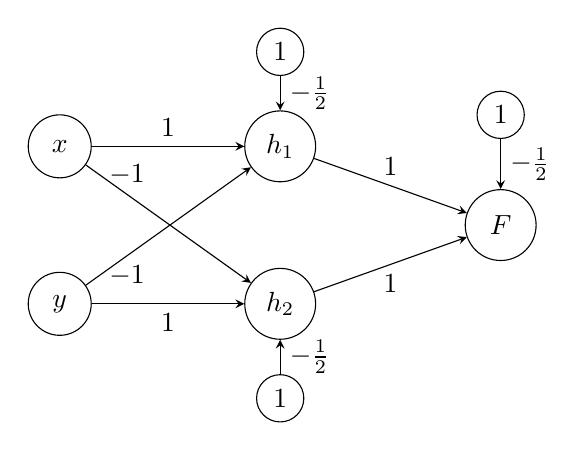
\begin{tikzpicture}[>=stealth]
  \node[draw,circle,minimum size=8mm] (x) at (0,1) {$x$};
  \node[draw,circle,minimum size=8mm] (y) at (0,-1) {$y$};
  \node[draw,circle,minimum size=9mm] (h1) at (2.8,1) {$h_1$};
  \node[draw,circle,minimum size=9mm] (h2) at (2.8,-1) {$h_2$};
  \node[draw,circle,minimum size=9mm] (f) at (5.6,0) {$F$};
  \node[draw,circle,minimum size=6mm,inner sep=0pt] (b1) at (2.8,2.2) {$1$};
  \node[draw,circle,minimum size=6mm,inner sep=0pt] (b2) at (2.8,-2.2) {$1$};
  \node[draw,circle,minimum size=6mm,inner sep=0pt] (bf) at (5.6,1.4) {$1$};

  \draw[->] (x) -- node[pos=0.5,above] {$1$} (h1);
  \draw[->] (x) -- node[pos=0.25,above] {$-1$} (h2);
  \draw[->] (y) -- node[pos=0.25,below] {$-1$} (h1);
  \draw[->] (y) -- node[pos=0.5,below] {$1$} (h2);
  \draw[->] (h1) -- node[pos=0.5,above] {$1$} (f);
  \draw[->] (h2) -- node[pos=0.5,below] {$1$} (f);
  \draw[->] (b1) -- node[pos=0.5,right] {$-\frac12$} (h1);
  \draw[->] (b2) -- node[pos=0.5,right] {$-\frac12$} (h2);
  \draw[->] (bf) -- node[pos=0.5,right] {$-\frac12$} (f);
\end{tikzpicture}
\end{center}
Les trois entrées constantes $1$ représentent les biais de valeur $-1/2$.
Il donne respectivement $0,1,1,0$ sur $(0,0),(1,0),(0,1),(1,1)$, comme demandé.}
\end{enumerate}
}
